\documentclass[reprint,english,notitlepage]{revtex4-2}

\usepackage[utf8]{inputenc}
\usepackage[english]{babel}

\usepackage{physics,amssymb}
\usepackage{graphicx}
\usepackage{xcolor}
\usepackage{hyperref}
\usepackage{tikz}
\usepackage{listings}
\usepackage{subfigure}
\usepackage{placeins}
\usepackage{hyperref}
\graphicspath{ {/Users/rebeccanguyen/Documents/GitHub/H22} }

\hypersetup{
    colorlinks,
    linkcolor={red!50!black},
    citecolor={blue!50!black},
    urlcolor={blue!80!black}}


\lstset{
	inputpath=,
	backgroundcolor=\color{white!88!black},
	basicstyle={\ttfamily\scriptsize},
	commentstyle=\color{magenta},
	language=Python,
	morekeywords={True,False},
	tabsize=4,
	stringstyle=\color{green!55!black},
	frame=single,
	keywordstyle=\color{blue},
	showstringspaces=false,
	columns=fullflexible,
	keepspaces=true}

\begin{document}
\title{Temperfect mug}   % self-explanatory
\author{Rebecca Nguyen}               % self-explanatory
\date{\today}                             % self-explanatory
\noaffiliation
\maketitle                                % creates the title, author, date & abstract


% the fundamental components of scientific reports:
\section{Introduction}
In this experiment we want to study the temperature of a liquid in two thermos mugs; Bodum and Temperfect.
Bodum mug is a regular thermos cup. The Temperfect mug removes excess heat from your beverage and stores it in its walls. This allows the newly-brewed beverage to
be enjoyed right away. Temperfect add an extra layer of insulation which changes from solid to liquid as it absorbs heat. Thereafter, the heat is added back into the beverage and is used to keep it a perfect temperature. During this phase the material returns back to a solid state and the energy given up is called latent heat.
We will be looking at temperature development over time for both mug. Both in order to see if the mug works as advertised and discuss if Temperfect can be modelled as an Einstein solid.

\section{Theory}
The multiplicity in an Einstein solid is given by
\begin{equation}
  \Omega(N, q) = \frac{(q+N -1)!}{q! (N -1)!} \approx \frac{(q+N)!}{q!N!}
\end{equation}
where q is number of energy units $\epsilon$ and N is number of oscillators. The expression has been further simplified using Stirling's approximation. We have considered the case q $\gg$ N (when there are
more energy units than oscillators, the so-called 'high-temperature' limit) in order to simplify it.
This further gives us the expression for entropy
\begin{equation}
  S \equiv k \ln\Omega
\end{equation}
where k is Boltzmann's constant.
Internal energy of an Einstein solid is given by

\begin{equation}
  U = \frac{N}{2}\epsilon + q\epsilon
\end{equation}

Which results in
\begin{equation}
  \frac{dU}{dq} = \epsilon \rightarrow dU = \epsilon dq
\end{equation}
with variations in.\\

One of the most important identities in thermal dynamics, derived from the first law of thermodynamics, is as follows
\begin{equation}
dU = Tds - Pdv \\
\end{equation}
We assume constant pressure and volume which allows us to rewrite the equation as
\begin{equation}
  dU = Tds \rightarrow T = \frac{dU}{dS} = \frac{\epsilon dq}{dS}
\end{equation}
Numerically we find this as
\begin{equation}
  T_i = \epsilon\frac{q_i - q_{i -1}}{S_i - S_{i -1}}
\end{equation}
\\
Lastly we have heat capacity
\begin{equation}
C_v = \frac{dU}{dT} = \frac{\epsilon dq}{dT}
\end{equation}
Numerically we find this as
\begin{equation}
  C_{v, i} = \epsilon\frac{q_i - q_{i -1}}{T_i - T_{i -1}}
\end{equation}

Temperature of the water changes due to heat flux to its surroundings or air
\begin{equation}
  AJ_q = \frac{dQ}{dt} = mc_v\frac{dT}{dt}
  \label{eq: heatflux}
\end{equation}
A is the area which heat flux takes place. Q, m and $c_V$ are attributes of the water (heat, mass and heat capacity).\\
Heat loss can be expressed as
\begin{equation}
  \frac{\Delta{T}}{\Delta{T_0}} = \exp(-t/\tau)
  \label{eq: heatloss}
\end{equation}
$\Delta{T} = T_w - T_a$ is the temperature difference between the water and air. Subscripts 0 describes initial state, t is time and $\tau$ is a time constant.
\section{Method}
The Temperfect mug and Bodum thermos cup were both filled with 3dl of almost boiling water. The lids were not put on to allow temperature logging while the water in the mugs cooled. The temperature in the air outside of the mug was $T_a = 22^{\circ}$.
\begin{figure}[!htb]
  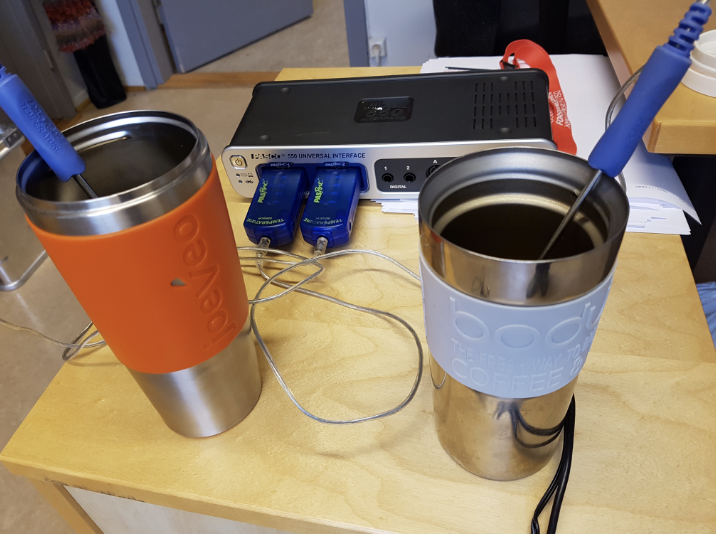
\includegraphics[scale=0.5]{setup.png}
  \caption{Experimental setup for comparing the Temperfect and Bodum mug}\label{fig:setup}
\end{figure}
\FloatBarrier

\section{Results}
\begin{figure}[h]
  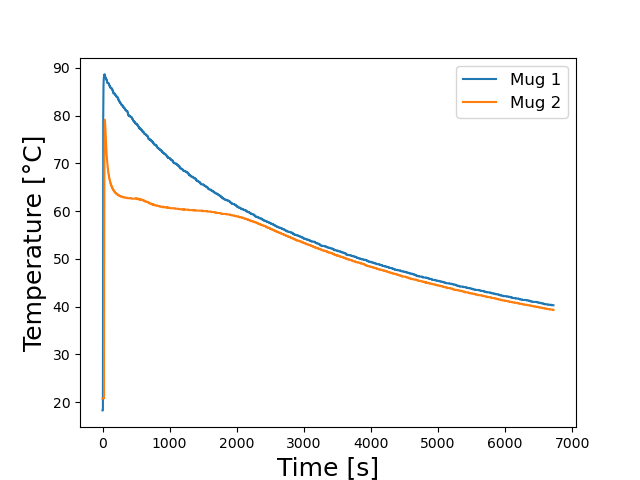
\includegraphics[scale=0.5]{temp.png}
  \caption{Temperature against time of both mugs}\label{fig:temperature}
\end{figure}
In figure (\ref{fig:temperature}) we have plotted temperature of both thermal mugs against time. Based on this figure we can conclude with Temperfect being mug 2 and Bodum being mug 1. The reasoning for this is mug 2's ability to bring the beverage temperature from almost boiling to a comfortable temperature rather fast. This is because the material absorbs the heat and goes through a phase transition: from a solid to a liquid. This melting temperature $T_m$ happens at around 60$^{\circ}$ during the period 0-200s.
Also, Temperfect (based on the orange graph) allows the temperature to stay in the so-called 'Ahhh zone'\footnote{A term for a comfortable drinking temperature used in this article describing \href{https://joeveo.com/pages/the-temperfect-mug}{Temperfect Technology}} for a longer period. During this phase the material puts its stored heat back into the beverage and returns back to a solid. This crystallising happens at around 700-2000s.
When the material in the mug is all solid, the temperature drops as if it was a regular mug.
Bodum on the other, steadily loses the heat of the beverage to the environment. This means the beverage takes longer time to reach a comfortable temperature, but will not stay there for long before the beverage is too cool.
The mathematical explanation behind the Temperfect is based on heat flux. Temperature of water changes due to heat flux, which is related to temperature gradient (\ref{eq: heatflux}). By storing heat in the walls of the cup and later re-introduce it back into the beverage reduces the heat flux.





\begin{figure}[h]
  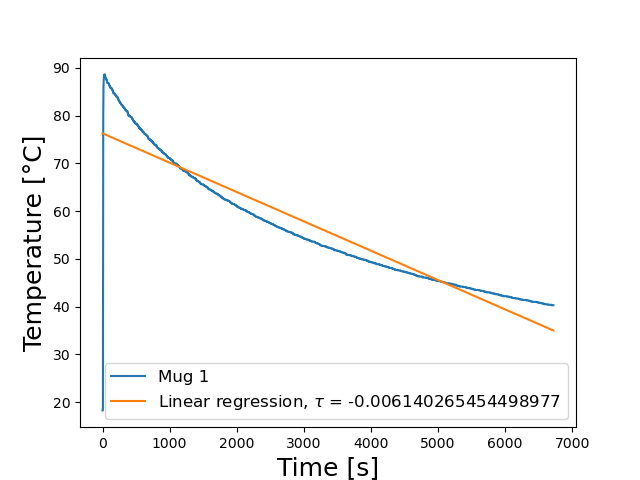
\includegraphics[scale=0.5]{tau_t.png}
  \caption{Model fitting using linear regression for mug 1}\label{fig:tau_t}
\end{figure}


\begin{figure}[h]
  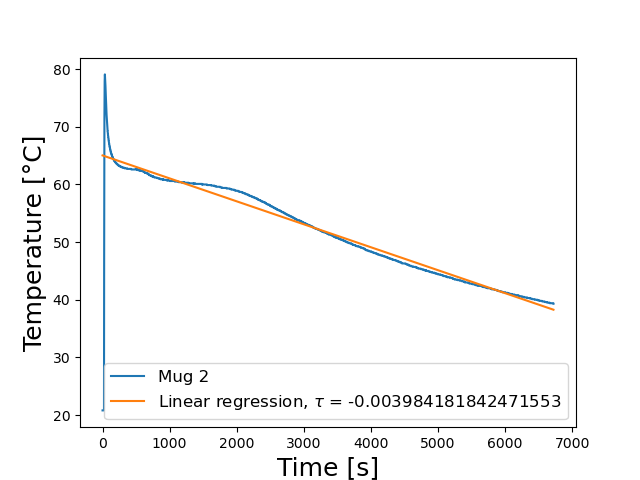
\includegraphics[scale=0.5]{tau_b.png}
  \caption{Model fitting using linear regression for mug 2}\label{fig: tau_b}
\end{figure}

Our attempt of model fitting the temperature gradient using linear regression, is shown in figure (\ref{fig:tau_t}) and (\ref{fig: tau_b}). $\tau$ describes rate of heat loss when looking at equation (\ref{eq: heatloss}). From this we were able to obtain values of $\tau$ for both mugs. However, this model does not describe our temperature model well. As seen from the figures, the model is just alright fiting for Temperfect, but completely wrong for Bodum.

\begin{figure}[h]
  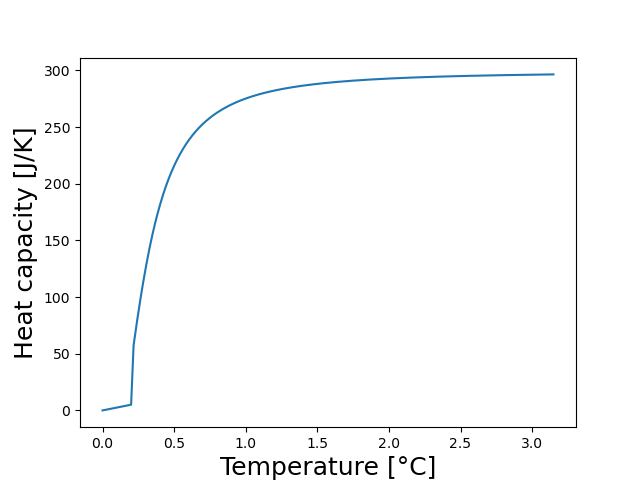
\includegraphics[scale=0.5]{T_mot_cv.png}
  \caption{Temperature against heat capacity for an Einstein solid}\label{fig: tagainstcv}
\end{figure}
When modelling the heat capacity related to temperature (for an Einstein solid) we discover one important attribute. As the temperature increases it becomes harder to heat up the material. This prevents the material from absorbing all the heat from the beverage. The system rather creates thermal equilibrium between the material and beverage. This attribute allows the material to only extract excess heat and occasionally re-introduce it back into the beverage. This happens as long as there is heat stored in the material.

\section{Discussion and conclusion}
Einstein solid can be used to model the Temperfect mug. The model describe how the material in the mug absorbs and stores heat in its wall. As well as explain the thermal equilibrium between the beverage and material as temperature increases. In conclusion the model describe the mug as advertised.
However, I am not sure it the model is sufficient. In my algorithm I have only considered the case of 'high-temperature' so I am not able to describe the solid for lower temperature. My algorithm seems to also have an error regarding the values on the axis of figure (\ref{fig: tagainstcv}), which does not make physical sense. The graph itself does physical sense.

\newpage
%% if you want to include an appendix, this is how you do it
\appendix
\section{Concept questions}
1. A thermos bottle with a piston instead of a lid contains a fixed amount of gas. Because it is a thermos
bottle, no heat can enter or leave the bottle. The
piston is then pushed in, compressing the gas. \\
(a) Does the pressure of the gas increase, decrease,
or stay the same?\\
As the piston push down, the pressure increases. That is because we decrease the volume where the gas molecules take place.\\
(b) Does the temperature of the gas increase, decrease, or stay the same?\\
As the pressure increases, the temperature also increases. Not sure if we assume an ideal gas, but I believe the reasoning is the same for all gases. For now we will look at ideal gas law: $PV = nkT$. As we can observe, increasing pressure result in higher value on the left-hand side of the equation. This result in a higher value on the right-hand side as well.\\
(c) Describe the behaviour of the molecules of gas
during the compression and support your answers to (a) and (b) with an explanation in
terms of their behaviour. \\
There is an increase in kinetic energy of the molecules as a consequence of increased pressure and temperature.\\
(d) Are there an other properties of the gas that
change?\\
Change of entropy of the gas.\\

2. Consider the same system except now the bottle
allows heat to go in or out of the bottle. The piston
is moved slowly, and the temperature of the gas is
maintained constant.\\
(a) In terms of what is happening to the
molecules, how is this situation different from
the situation in the first question?\\
As there is no increase in temperature and some gas escape, the molecules will not be having an increase in kinetic energy in this situation.
(b) Does the pressure of the gas increase, decrease,
or stay the same?\\
The pressure stay the same since some of the gas escape as the piston moves slowly and there is no increase in temperature.
(c) Support your answer to (b) with an explanation in terms of what is happening to the
molecules of gas.\\
Some gas escape, meaning some molecules escape. The temperature and pressure does not increase and the motion of molecules remains the same.
(d) Are there any other properties of the gas that
change?\\
No change in entropy.


\section{Code}
\begin{lstlisting}[language=Python]
import numpy as np
import matplotlib.pyplot as plt
import os
import scipy.stats as sc
import random
from math import factorial
import scipy.constants as scc

time = [] # [s]
T_t = [] # Temperature of water inside Temperfect mug
T_b = [] # Temperature of water inside bodum thermos mug

# read termokopper.txt and store data in arrays
with open('termokopper.txt', 'r') as lines:
    for line in lines:
        row = line.split()
        time.append(float(row[0]))
        T_t.append(float(row[1]))
        T_b.append(float(row[2]))

time = np.array(time)
T_t = np.array(T_t)
T_b = np.array(T_b)

###### Calculate tau of both mugs  ##########

slope_t, intercept_t, r_t, p_t, se_t = sc.stats.linregress(time, T_t)
slope_b, intercept_b, r_b, p_b, se_b = sc.stats.linregress(time, T_b)

###### Einstein solid  ##########

k = 1 #scc.Boltzmann
N = int(300) # a suitable numbers of oscillators
nsteps = 800
q = np.linspace(1, nsteps, nsteps) # number of energy units
dq = (q[-1]-q[0])/(len(q)-1)

omega = np.zeros(nsteps) # multiplicity of an Einstein solid
for i in range(nsteps):
    omega[i] = factorial(int(q[i]) + N - 1)/(factorial(int(q[i]))
    *factorial(N - 1))

S = k*np.log(omega) # entropy

dqdS = np.zeros(nsteps)
for i in range(1, nsteps):
    dqdS[i] = dq/(S[i] - S[i - 1])

T = dqdS # temperature

Cv = np.zeros(nsteps) # heat capacity
for i in range(1, nsteps):
    Cv[i] = dq/(T[i] - T[i -1])

###### Attempt on translating MATLAB code from appendix A ##########

Ctb = 5
N = 80000
nstep = 15*N
tau = N
Tt = np.zeros(nstep)
Tb = np.zeros(nstep)
Tt[0] = 1
Tb[0] = -1
Tr = -1

for i in range(1, nstep):
    r = random.uniform(-2, 2)
    DT = Tt[i - 1] - Tb[i - 1]
    if (r < DT):
        Tt[i] = Tt[i - 1] - 1/N
        Tb[i] = Tb[i - 1] + Ctb/N
    else:
        Tt[i] = Tt[i-1] + 1/N
        Tb[i] = Tb[i-1] - Ctb/N

plt.plot(np.linspace(0, nstep, nstep)/tau, Tt, "r")
plt.plot(np.linspace(0, nstep, nstep)/tau, Tb, "k")
plt.show()

# Temperature plot over time of both mugs
"""
plt.plot(time, T_t, label = "Mug 1")
plt.plot(time, T_b, label = "Mug 2")
plt.xlabel("Time [s]", fontsize = 18)
plt.ylabel("Temperature [°C]", fontsize = 18)
plt.legend(prop={'size': 12})
plt.savefig("temp.png")
plt.show()
"""

# Plot tau of Temperfect
"""
plt.plot(time, T_t, label = "Mug 1")
plt.plot(time, slope_t*time + intercept_t, label = rf"Linear regression,
$\tau$ = {slope_t}")
plt.xlabel("Time [s]", fontsize = 18)
plt.ylabel("Temperature [°C]", fontsize = 18)
plt.legend(prop={'size': 12})
#plt.savefig("tau_t.png")
plt.show()
"""

# Plot tau of Bodun
"""
plt.plot(time, T_b, label = "Mug 2")
plt.plot(time, slope_b*time + intercept_b, label = rf"Linear regression,
 $\tau$ = {slope_b}")
plt.xlabel("Time [s]", fontsize = 18)
plt.ylabel("Temperature [°C]", fontsize = 18)
plt.legend(prop={'size': 12})
plt.savefig("tau_b.png")
plt.show()
"""

# plot T against S
"""
plt.plot(T, S)
plt.xlabel("Temperature [°C]", fontsize = 18)
plt.ylabel("Entropy [J/K]", fontsize = 18)
plt.savefig("T_mot_S.png")
plt.show()
"""

# plot T against Cv
"""
plt.plot(T, Cv)
plt.xlabel("Temperature [°C]", fontsize = 18)
plt.ylabel("Heat capacity [J/K]", fontsize = 18)
plt.savefig("T_mot_cv.png")
plt.show()
"""

#print(os.getcwd())
\end{lstlisting}
\end{document}
